\documentclass[a4paper,10pt]{article}
\usepackage[utf8]{inputenc}
\usepackage[spanish]{babel}
\usepackage[affil-it]{authblk}
\usepackage{enumerate}
\usepackage{graphicx}
\usepackage{hyperref}
\usepackage{amsmath}
\usepackage{amssymb}



%opening
\title{Mecánica Clásica Tarea \# 1}
\author{Favio Vázquez\thanks{Correo: favio.vazquezp@gmail.com}}\affil{Instituto de Física. Universidad Nacional Autónoma de México}
\date{}

\begin{document}

\makeatletter
\def\@maketitle{%
  \newpage
  \null
  \vskip 2em%
  \begin{center}%
  \let \footnote \thanks
    {\Large\bfseries \@title \par}%
    \vskip 1.5em%
    {\normalsize
      \lineskip .5em%
      \begin{tabular}[t]{c}%
        \@author
      \end{tabular}\par}%
    \vskip 1em%
    {\normalsize \@date}%
  \end{center}%
  \par
  \vskip 1.5em}
\makeatother

\maketitle

1.- Encontrar el movimiento de un oscilador armónico amortiguado
con un coeficiente de amortiguamiento de $\gamma = \omega_{0}/3$ 
($\omega_{0}/3$ frecuencia natural de l oscilador) si a $t=0$ está 
en reposo en su punto de equilibrio y a partir de ese instante se le
aplica una fuerza dada por $$F=A\sin{\omega_{0}t}+B\sin{3\omega_{0}t}$$

\underline{Solución:}

\vspace{.3cm}

2.- Considere un oscilador armónico con un pequeño amortiguamiento.
Muestre que el cambio en la energía durante un período es $2T/\tau$,
donde $T$ el período de oscilador sin amortiguar y $\tau$ es el tiempo
que tarda la amplitud en reducirse por un factor $1/e=1/2,718$.

\vspace{.3cm}

\underline{Solución:}

\vspace{.3cm}

3.- Un proyectil se dispara a partir del origen con velocidad inicial $v_{0}$.
Se desea impactar el punto de coordenadas $x=x_{0}$, $z=0$.

\begin{enumerate}[a)]
 \item ¿Cuál es el ángulo (o ángulos) de disparo que se requieren?
 \item Encuentre la corrección a primer orden que se debe dar a dicho ángulo si toma 
 en cuenta la resistencia del aire.
\end{enumerate}
\vspace{.3cm}

\underline{Solución:}

\vspace{.3cm}

Podemos esquematizar el problema como en la (figura \ref{fig:problema3}). 
Tenemos un proyectil que es disparado desde el origen a una velocidad 
inicial $v_0$, haciendo un ángulo $\theta$ con el eje x, y deseamos
alcanzar el punto $x=x_0$ y $z=0$. Primero consideremos el caso sin
tomar en cuenta la resistencia del aire.

\begin{figure}[ht]
 \centering
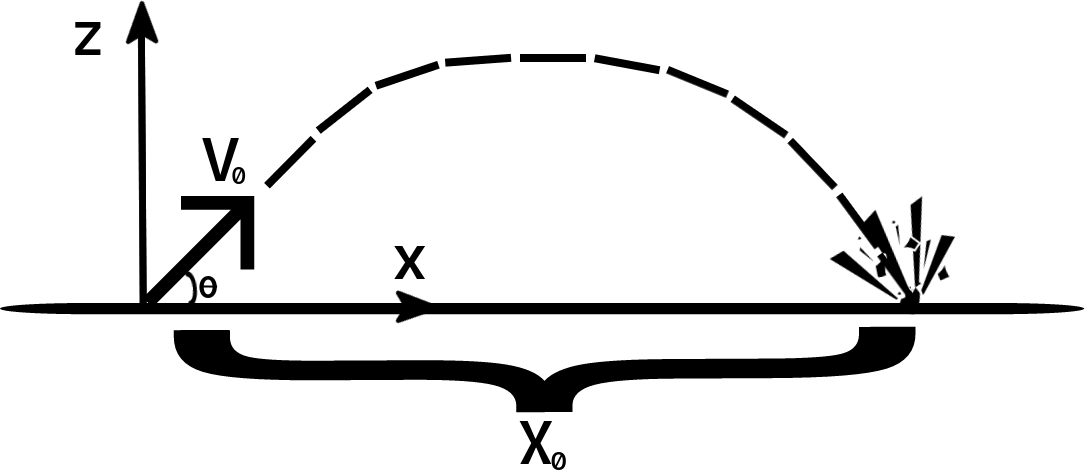
\includegraphics[scale=0.3]{problema3fig1}
\caption{Problema 3}
\label{fig:problema3}
\end{figure}

\vspace{.3cm}

De la (figura \ref{fig:problema3}) utilizando las relaciones trigonométricas en un 
triángulo rectángulo vemos que

\begin{gather*}
v_{0x} = v_0\cos(\theta) \\
v_{0z} = v_0\sen(\theta)
\end{gather*}


Si la partícula de masa $m$ está sujeta a la atracción gravitacional
por la tierra, entonces tenemos, utilizando la segunda ley de Newton,

\vspace{.3cm}

En la dirección de $x$,

\begin{equation}
 0 = m \ddot{x}
 \label{ec:1}
\end{equation}

y en la dirección de $z$,

\begin{equation}
 - mg = m \ddot{z}
  \label{ec:2}
\end{equation}

De la ecuación (\ref{ec:1}) tenemos que (utilizando las condiciones iniciales),

\begin{equation*}
 \ddot{x} = 0 \Rightarrow \frac{d\dot{x}}{dt} = 0 \Rightarrow 
 \int_{v_{0x}}^{\dot{x}}d\dot{x}' = 0 \Rightarrow \dot{x} - v_{0x} = 0 
 \end{equation*}

\begin{equation}
 \therefore \dot{x} = v_0 \cos(\theta)
 \label{eq:3}
\end{equation}

De la ecuación (\ref{eq:3}) podemos obtener $x(t)$, 

\begin{equation*}
 \frac{dx}{dt} = v_0 \cos(\theta) \Rightarrow dx = v_0 \cos(\theta) dt \Rightarrow
 \int_0^x dx' = v_0 \cos(\theta) \int_0^t dt'
\end{equation*}

\begin{equation}
 \therefore x = v_0 t \cos(\theta)
 \label{eq:4}
\end{equation}

Luego para $z$, utilizando la ecuación (\ref{ec:2}),

\begin{equation*}
 \ddot{z} = -g \Rightarrow \frac{d\dot{z}}{dt} = -g \Rightarrow 
 \int_{v_{0z}}^{\dot{z}}d\dot{z}' = -g \int_0^t dt' \Rightarrow \dot{z} - v_{0z} = -gt 
 \end{equation*}
 
\begin{equation}
 \therefore \dot{z} = -gt + v_0 \sen(\theta)
 \label{eq:5}
\end{equation}

De la ecuación (\ref{eq:5}) podemos obtener $z(t)$,

\begin{gather*}
 \frac{dz}{dt} = -gt + v_0 \sen(\theta) \Rightarrow dz = (-gt + v_0 \sen(\theta)) dt \\ \Rightarrow
 \int_0^z dz' = -g\int_0^t t' dt' + v_0 \cos(\theta) \int_0^t t'dt'
\end{gather*}

\begin{equation}
 \therefore z = - g \frac{t^2}{2} + v_0 t \sen(\theta)
 \label{eq:6}
\end{equation}

Podemos encontrar el rango máximo de distancia que recorrerá el proyectil, 
es decir hasta que choque con el piso, cuando llegue al punto que hemos llamado
$x_0$, lo cual ocurre al final de su recorrido cuando $z=0$. Para dar
respuesta a la parte $a)$ de la pregunta debemos determinar en qué momento
esto ocurre, es decir cuánto es el valor del tiempo para el punto en que 
$z=0$, ya que esto nos permitirá determinar los ángulos de lanzamiento
que requerimos para que el proyectil llegue a $x_0$ y $z=0$.

\vspace{.3cm}

Debido a que el proyectil sale disparado desde el origen, $z=0$ cuando
$t=0$, pero mediante la ecuación (\ref{eq:6}) podemos determinar el otro
momento en que $z=0$ que es al final de su recorrido, y a este tiempo
lo llamaremos $\tau$, reescribiendo (\ref{eq:6}) podemos ver esto claramente,

\begin{equation*}
 z = t(\frac{-gt}{2} + v_0 \sen(\theta)) = 0
\end{equation*}

Donde vemos que $z=0$ si $t=0$, pero también para un tiempo $\tau$,

\begin{equation*}
 \frac{-g\tau}{2} + v_0 \sen(\theta) = 0
\end{equation*}

Resolviendo para $\tau$,

\begin{equation}
 \tau = \frac{2v_0\sen(\theta)}{g}
 \label{eq:7}
\end{equation}

Entonces para obtener el rango del proyectil en $z=0$ cuando
$t=\tau$, sustituimos en (\ref{eq:4})

\begin{equation*}
 x = v_0 \tau \cos(\theta) \Rightarrow x = 2 \frac{(v_0)^2}{g} \sen(\theta)\cos(\theta)
\end{equation*}

Utilizando la identidad trigonométrica $2\sen(\theta)\cos(\theta) = \sen (2\theta)$,
obtenemos que

\begin{equation}
 x = \frac{(v_0)^2}{g} \sen(2\theta)
 \label{eq:8}
\end{equation}

El rango será máximo, es decir el proyectil llegará a $x_0$ y $z=0$ para
la familia de ángulos $\theta$ que hagan que $\sen(2\theta)=1$, tales
ángulos son:

\begin{equation}
 \theta = \frac{n\pi}{4} \qquad \qquad n = 4\epsilon - 3, \quad  \epsilon = 1,2,3,4,5,\dots
 \label{eq:9}
\end{equation}

















\vspace{.3cm}

4.- Dos partículas de masa $m_1$ y $m_2$ están amarradas por una cuerda sin masa de 
longitud $l$ y descansan sobre una mesa sin fricción. En el instante t=0 la cuerda
está totalmente desplegada y las masas están en reposo; en ese instante se le aplica
un impulso a la partícula $m_2$ de tal suerte que ésta adquiere una velocidad $v_0$ 
perpendicular a la cuerda.

\begin{enumerate}[a)]
 \item Describa el movimiento después de haber aplicado el impulso
 \item ¿Cuál es la tensión de la cuerda durante el movimiento?
\end{enumerate}

\vspace{.3cm}

\underline{Solución:}

\vspace{.3cm}

5.- Una partícula de masa $m_1$ tiene una energía cinética $T_1i$ y choca elásticamente 
con otra de masa $m_2$. La segunda partícula sale disparada en una dirección que hace un
ángulo $\theta$ con la dirección del movimiento inicial de la primera partícula. Encuentre
la energía cinética $T_2f$ con la que sale la segunda partícula. Muestre que esta energía
es máxima si el choque es de frente.

\vspace{.3cm}

\underline{Solución:}

\vspace{.3cm}

6.- Un objeto de masa $m$ se encuentra en el ecuador de la Tierra. ¿Qué velocidad debe 
tener para que su peso y la fuerza de Coriolis sean iguales?

\vspace{.3cm}

\underline{Solución:}

\vspace{.3cm}

7.- La hélice de un avión tiene un momento de inercia $I$ y el motor le imprime una torca 

$$N_m = N_0 (1+\alpha \cos{\omega t}. \qquad (\alpha \ll 1)$$

La resistencia del aire le imprime una torca

$$N_f = -b\dot{\theta}$$

¿Cuál es el estado estacionario del movimiento de la hélice?

\vspace{.3cm}

\underline{Solución:}

\vspace{.3cm}

8.- Dos cuerpos rígidos extensos (no puntuales) chocan elásticamente. ¿Es posible que 
después del choque ambos queden únicamente con energía cinética de rotación en torno 
a sus centros de masa?. De ser así de un ejemplo.
\vspace{.3cm}

\underline{Solución:}

\vspace{.3cm}
9.- Un meteorito choca con la Tierra en el Polo Norte haciendo un ángulo $\theta$ con
el eje de la tierra. El meteorito tiene una masa igual a $1/10^-17$ de la masa de la 
Tierra y llega con la velocidad de escape. ¿En qué forma se verá perturbado el movimiento
de rotación de la Tierra? (Desprecie el cambio en el momento de inercia de la Tierra
debido a la incrustación del meteorito).
\vspace{.3cm}

\underline{Solución:}

\vspace{.3cm}

10.- Uno de los postulados básicos de la mecánica clásica es el de la relatividad galileana,
nos dice que la mecánica clásica debe ser invariante ante las transformaciones de Galileo, 
esto es las leyes de la física básica deben ser las mismas en todos los sistemas inerciales
de referencia y la transformación entre un sistema inercial y otro es la de Galileo 
($\hat{r}' = \hat{r} - \hat{v}'t$ donde $\hat{v}'$ es la velocidad constante entre los dos 
sistemas de referencia).

\begin{itemize}
 \item En la formulación de Newton de 1687 se consideraba la existencia de un sistema 
 absoluto de referencia que permitía definir el estado de reposo de un cuerpo, Newton lo
 veía como un sistema anclado a las estrellas fijas o uno muy cercano a este. La visión 
 moderna se desarrolló en el siglo XIX, elimina la idea del reposo absoluto y hace 
 uso del postulado que mencionamos. Describa brevemente el cambio entre la visión 
 estrictamente newtoniana y la del siglo XIX.
 \item Muestre, a manera de ejemplo del cumplimiento del postulado anterior, que las 
 ecuaciones de movimiento del oscilador armónico tridimensional son invariantes ante
 las transformaciones de Galileo.
\end{itemize}

\vspace{.3cm}

\underline{Solución:}

\vspace{.3cm}

\end{document}
